\chapter{Applications and Results}
{\color{red} 
Investigation of constraints impact in time windows was performed by analyze in two different type of association networks; the networks with fixed step size nodes and the networks with fixed bucket size nodes.

Those two different type of networks were applied in all 10 time windows and average modularity metric plots were generated. 
}
\section{Data Cleaning}
{\color{red}
	Upon to two distinctive constraint definitions in my advance project 2 report, checking those hypothetical terms in real life data is decided. To be able to observe interesting patterns, a big data set with 2-3 years production orders is agreed to be investigated through time windows. 

After discussing the relevant features to be considered in this data set, below given SQL query was generated to pull the data set from the SMS database. The resultant data set consists of 459203 rows and 15 columns. 

First two columns and $4^{th}$ column features: ROS.R\_OS\_ID, ROS.PRODUCTION\_LINE\_NAME, and ROS.REFERENCE\_DATE come from "Reporting data: Operation step" table. $3^{rd}$ column feature SEQUENCE\_ID is actual casting sequence ID from the table "Reporting data: additional data of CCM (explain this)". $5^{th}$., $6^{th}$., $7^{th}$. and $14^{th}$. SLAB.PIECE\_ID, SLAB.MATERIAL\_ID, SLAB.MOLD\_WIDTH, and SLAB.EXIT\_TEMP come from "Reporting data: additional data of CCM which are slab related". Rest of the columns: MAT.WIDTH, MAT.THICKNESS, MAT.WEIGHT, MAT.LENGTH, MAT.HEAR\_ID, MAT.STEEL\_GRADE\_ID\_INT, and MAT.SLAB\_TRANSITION come from "Material ;  For slabs, coils, plates and heats" table.

\begin{lstlisting}
SELECT  ros.r_os_id, ros.production_line_name, ccm.sequence_id,        
ros.reference_date, NVL( TO_CHAR(slab.piece_id),'NA') 
piece_id, NVL( TO_CHAR(slab.material_id),'NA') material_id, 
NVL(TO_CHAR(slab.mold_width),'NA') mold_width, 
NVL( TO_CHAR(mat.width),'NA') width, 
NVL( TO_CHAR(mat.thickness),'NA') thickness, 
NVL( TO_CHAR(mat.weight),'NA') weight, 
NVL( TO_CHAR(mat.length),'NA')
length, NVL( TO_CHAR(mat.heat_id),'NA') heat_id, 
NVL( TO_CHAR(mat.steel_grade_id_int),'NA') steel_grade_id_int, 
NVL( TO_CHAR(slab.exit_temp),'NA') exit_temp, 
NVL( TO_CHAR(mat.slab_transition),'NA') slab_transition
	
FROM   	L3MAIN.r_os ros 
LEFT JOIN L3MAIN.r_ccm ccm ON ros.r_os_id = ccm.r_os_id 
LEFT JOIN L3MAIN.r_ccm_slab slab ON ros.r_os_id = slab.r_os_id 
LEFT JOIN L3MAIN.r_mat mat ON ros.r_os_id = mat.r_os_id 
	
WHERE  	sequence_id IS NOT NULL;
\end{lstlisting}

Parsed data belongs to CCM (Continuous Casting Machine) production line.

$7.85 g/cm^{3}$ = $7850 kg/m^{3}$ = $0.284 lb/in^{3}$ = $490 lb/ft^{3}$

Converting strings to numbers and correction for punctuation marks between digits were performed, null values (NA) were converted into $0$ values in the beginnning of data cleaning process. After completing minor stages, some preconditions were generated as below to be able to manipulate data columns.
Steel density is considered between $7.00 x 10^{-6}$ $kg/mm^{3}$ and $8.50x10^{-6}$ $kg/mm^{3}$.
Width varies between 800 - 2000 mm. 
Thickness varies between 40 - 90 mm. 
Weight varies between 2669 - 26690 kg.
Length unit is mm.

Starting to modify width, thickness, and weight values corresponding to thickness values with 2 digits.

The data set has below given shape just before starting to analysis.
Weight Zero Rows: 10484
Thickness + Width + Weight Zero Rows: 61320
The rows with densities that do not match within above mentioned interval: 1787
Usable Rows: 396096

Time Windows Generation by Data Partitioning:

the dataset with length 396096 was partitioned in 10 time windows starting from the beginning of the data. In each step, it's increased by 39610 rows more or less (increasing windows). The exact increase step dimension was specified by the last order of corresponding sequence. For my dataset, exact time window lengths are 39871, 79567, 118358, 158421, 198041, 237352, 277147, 316411, 356385, 396096. Almost always same statistics for every window. Strange increase modularity increase towards the end due to increasing window size. If there is a shift in the way the data behave, I will almost not see it because it is mast by the other data that still be present in my analysis. The modularity curves seem drift upwards little bit. There is a trend of going up now matter how it behaves in the middle. My reason was to do this to check the load effect.

Partitioning was repeated with discrete time windows (sliding windows). Shifting window within equal windows size. To see the results of same analysis in each discrete time window. Whether the rules I discovered from the first dataset (1st time window) and the second dataset (2nd time window) are really fundamentally different or rather the same.

21.04.21
Below steps were performed for the data sets belong to different production lines.
•	Sequences with less than 50 events were removed from the data sets considering those short sequences might be generated for some test processes. 
•	The events with the densities out of the interval (6.5x10-6, 8.5x10-6) were removed from the data sets.

At the final stage, obtained data set lengths are given below.
\begin{itemize}
	\item PLTCM data set: 64,026 events
	\item CGL data set: 31,230 events
	\item CSP data set: 205,496 events
	\item CCM data set: 347,418 events
\end{itemize}
}

\section{Real-life Events Analysis}
{\color{red} 
The steel manufacturing data sets were analyzed in six different dimensions: Production Line, Production Constraints, Production Feature, Time, Network Resolution and Null Model.

For the first dimension, distinguished data sets were considered among four different production line: Continuous Casting Machine (CCM), Compact Strip Production (CSP), Continuous Galvanizing Line (CGL), and Pickling Line \& Tandem Cold Mill (PLTCM). In principle, CCM and CSP production lines have similar functionalities; however, they were kept separated in the analysis pipeline since their labels are different in the database. Two fundamentally different constraints acting on the manufacturing process: technology-driven constraints and load-driven constraints, were shaped hypothetically and defined as two distinguished network approaches: fixed step-sized and fixed bucket-sized networks. Those attempts are in the second dimension of the analysis. As the third dimension, the width and thickness features of slabs were picked to investigate different production constraints that play a role in the machines for those features. Time is the fourth dimension and considered to check constraints impact on the historically ordered production events. The data set was treated in both discrete-time windows and increasing-time windows to study the behaviour of changing fixed step size and fixed bucket size. Generated networks were diversified in two different resolutions by changing the node amount in the fifth dimension. As a concept of characterizing, modularity was calculated for the networks. The aim is to keep the networks with a similar number of nodes in both network approaches (fixed step size and fixed bucket size) so that the modularity quantification would be meaningful to compare. As the last dimension, two types of null model: shuffling the links in degree conservation and shuffling them based on the communities, were considered to check the randomness of the networks. Obtained Z-scores can vary based on the generated null model via that specific randomization method.

The data sets were partitioned into two halves, and analysis steps were applied for the first half, second half, and the complete data set. At the top of bar chart sets, modularity values were presented for the original network and a single randomized network. Z-scores belong to different null models for 1000 randomized networks were given in the bottom part of the bar chart set, indicated with a colorless line finish. For each of the z-scores, error bars were included by removing and putting back 10\% of the data several times. The colored bar border indicates the mean value, and the T-shaped symbol represents the standard deviation of the error bars.
}

 \begin{figure}[!ht]
	\begin{center}
		\makebox[\textwidth]{
			\centering
			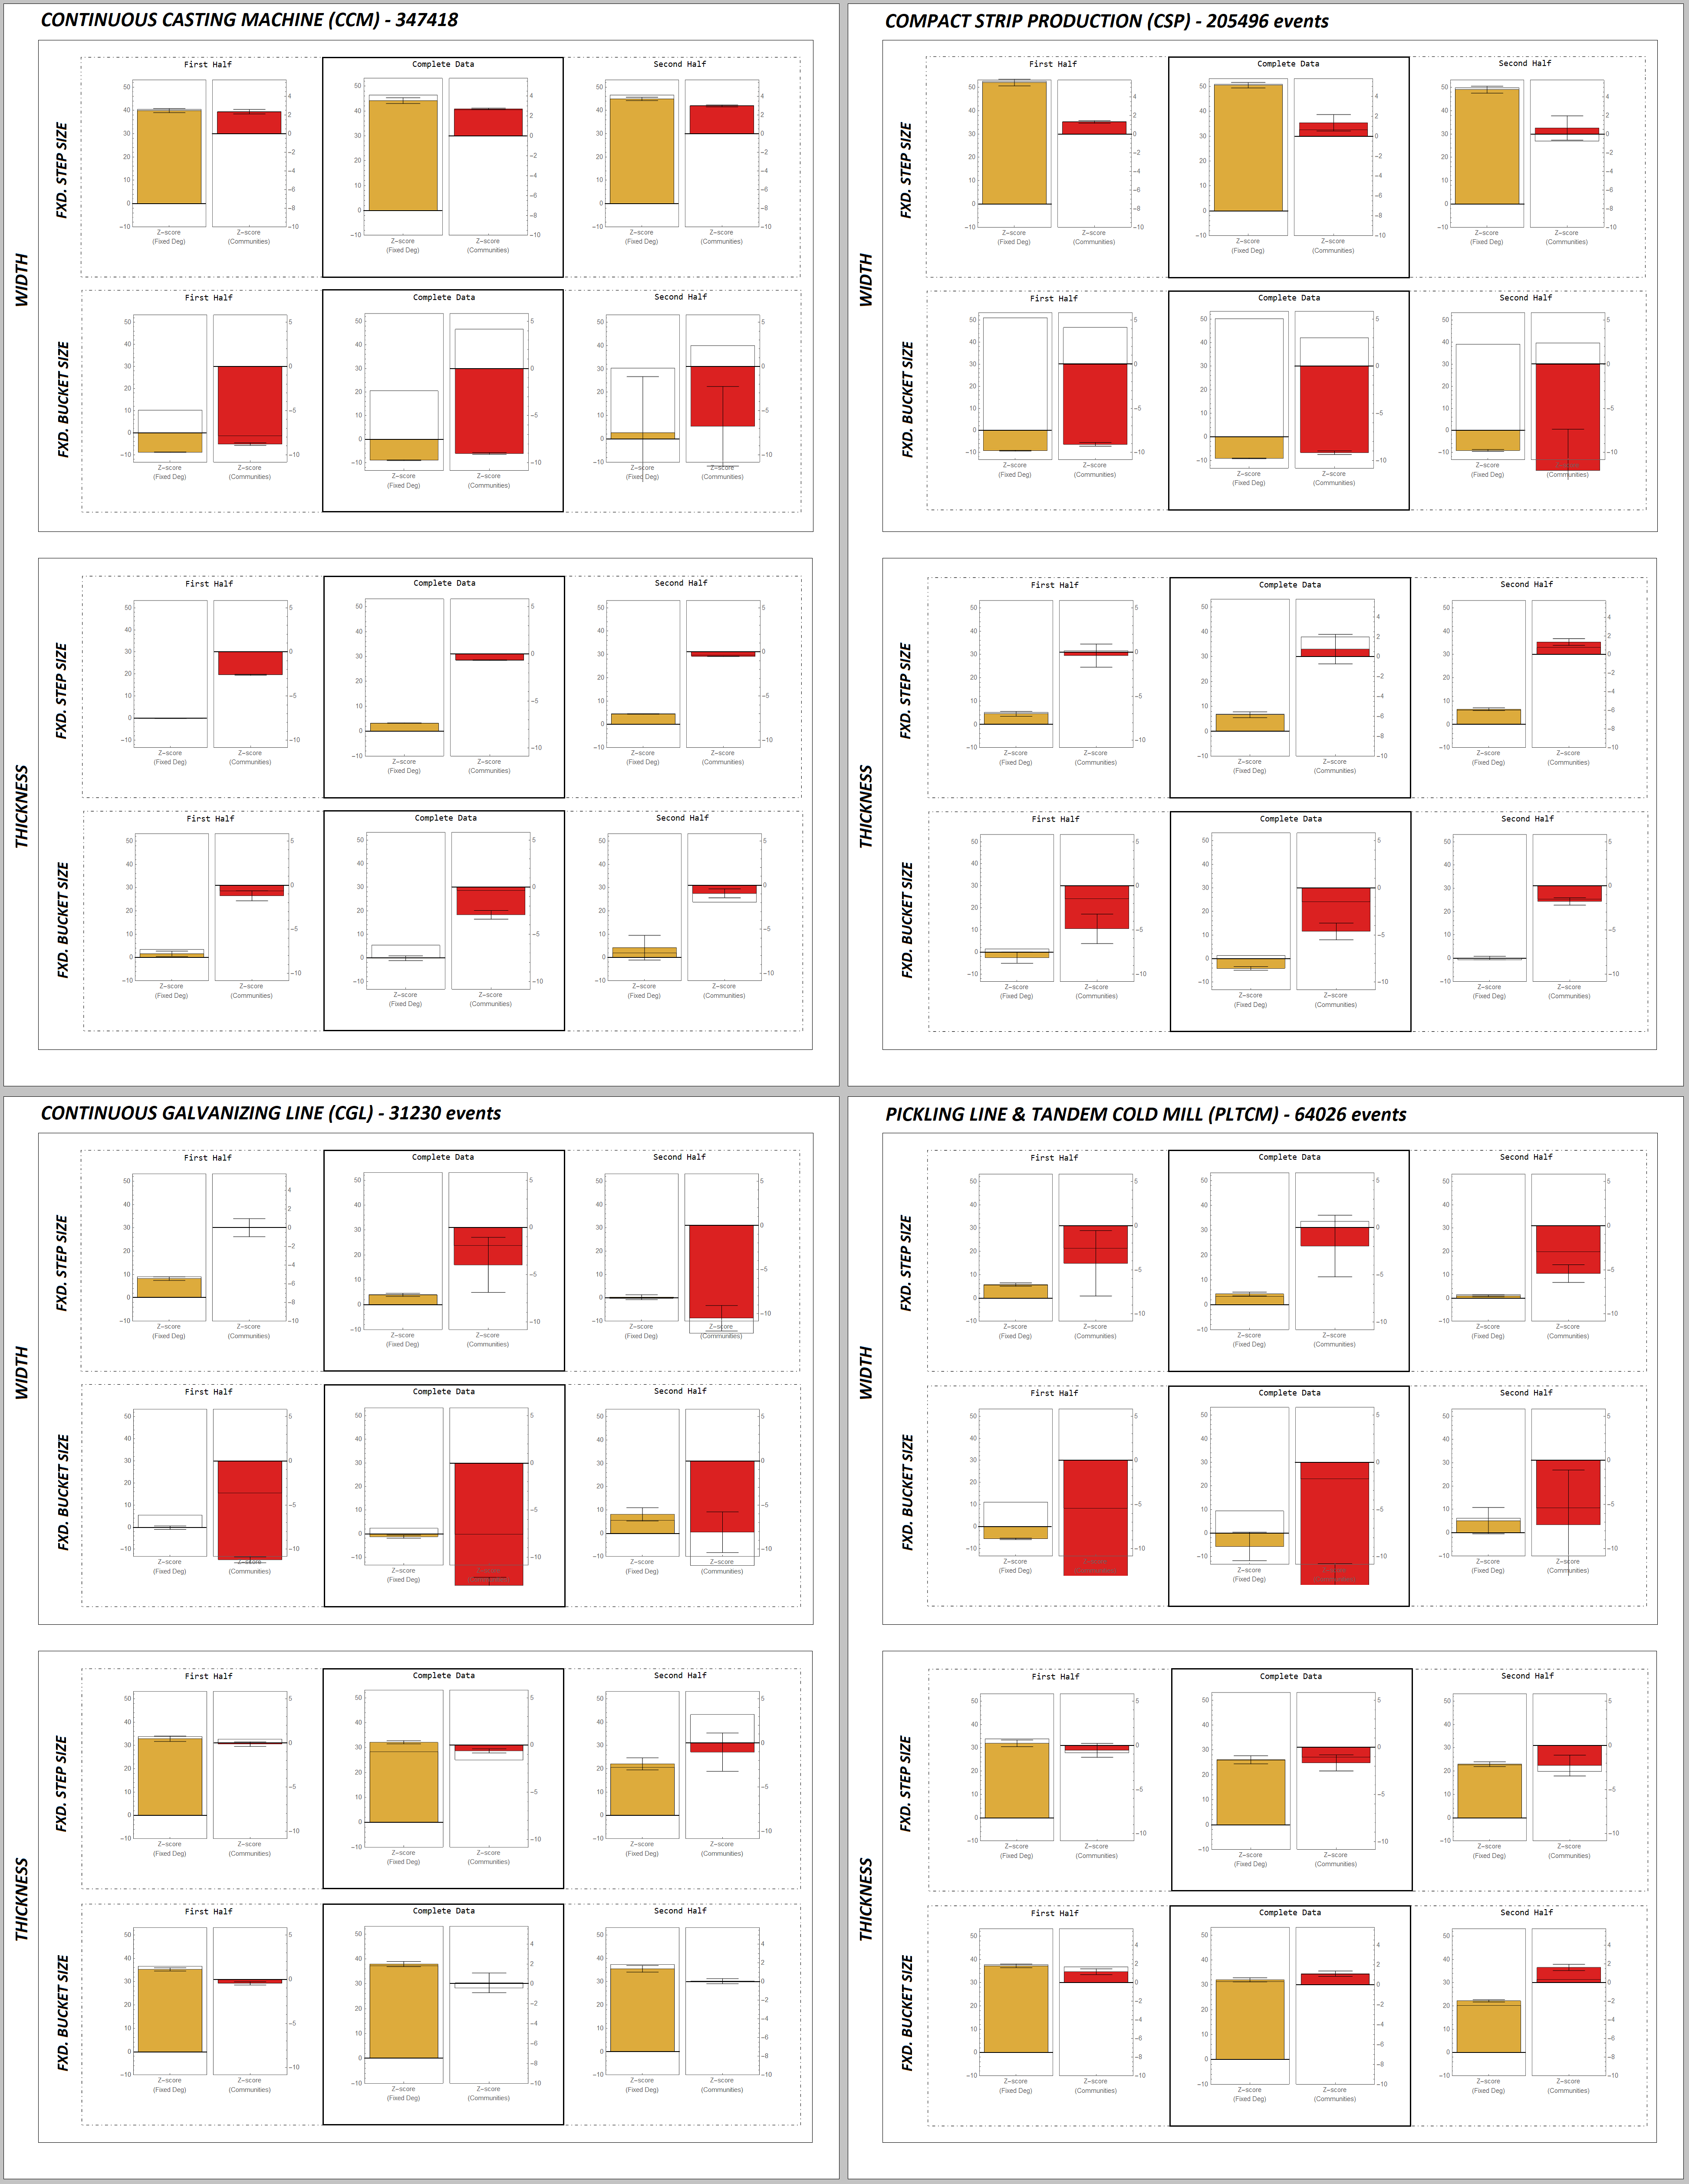
\includegraphics[width=1.05\linewidth]{../images/results-real_life_events_analysis-results.png}}
		\caption{CCM, CSP, PLTCM, CGL \aa{} Z-scores.}
		\label{figure-real-life-events-analysis-results}
	\end{center}
\end{figure}

{\color{red}
%	24.03.21
	Regarding behavior on networks with changing fss and fbs amounts, first column plots show a calibration curve which have graph node numbers corresponding to changing fss and fbs. For Weight feature, fbs paradigm leads to higher modularity than the fss paradigm no matter which bucket/step size we pick. This result becomes opposite when it comes to length and width. For thickness, there is no clear result to say as the others have. They are actually sometimes on the same level. The fact that modularity tends to be higher in one paradigm and lower in the other which is an interesting thing.
	
	Investigation of constraints impact in the data with time-resolved fashion confirms my previous investigation on the data with increasing time windows. 
	Our hypothesis at the moment is that the physical constraints are rather about step sizes than about bucket sizes. Because step size graphs are less random.
	
	In my previous project, the fixed step size graphs had a high modularity. This means that the actual quantity I discretize creates the constraints while in the case of fixed bucket size it would be the volume of orders that creates my constraints. This summarizes our hypothesis. 
	
%	What I would get = On the width level, we have a fairly constant behavior over time and it confirms what I see on the total dataset, strong difference in modularity between the two network approaches. For the fbs approach, there might be a transition, the fixed bucket size becomes very modular in the end.
	
	For thickness, its less clear because the modularity is in same level for both fss and fbs but the increase in modularity for fbs is fairly drammatic. It goes from 0.3 to 0.6 while the other remains at 0.3 and fluctuates. In the last two time windows in fbs, the process is dominated by something else. It is an evidence that something changed of the constraints involved really takes place.
	
%	For length, both modularity changes in different network structures are between 0.1 and 0.2 is beyond the resolution of what I can do. These two curves are almost identical in the statistical point of view. Also they are close to what you would get for totally random graphs in fact. There is no modularity here we can talk about.
	
%	For weight, it is same as length. The z-scores are fairly close to zero compare the ones for other feature z-scores. In the case of the fbs, you can see it might be slightly higher than the modularity of the random graphs but it is not a deservedly modularity.
	
	
	current situation
	The Modularity (Single Random Graph) and Z-score plots, dashed curves are provided for the Fixed Degrees Null Model and unbroken curves are provided for Modularity Null Model.
	Network node numbers were kept equal for the same time windows in different network approaches but not in the consecutive time windows in the same network approaches.
	Other than the below-given networks, including fewer nodes than 15 in some cases, all networks have varying node numbers between 25-90.
	\begin{itemize}
		\item CSP Thickness Network with narrow node binning
		\item CSP Thickness Network with large node binning
		\item CCM Thickness Networks with narrow and large node binning
	\end{itemize}

before treating time windows, having the modularity as function of bucket size and as function of step size. At this stage, choosing suitable step and bucket sizes and accordingly repeat all progress mentioned above. The aim is to obtain big amount of nodes as possible as we can and keeping that amount of nodes same in both graph structures (fixed step size and fixed bucket size). The difference between modularity values at highest graph nodes amount in fixed bucket and fixed step sized graphs shows which network structure is more effective on generating clear communities. In other words, modularity values is more meaningful when the node number is high.

Results are not stable which is a bit expected with these complicated data structures. This is why we do the sensitivity analysis on top of that: varying the resolution, doing things with slightly different methods (different null models) over and over again. 
%In some sense, we try to do the data as simpler as they are, by trying to pretend that they are more homogeneous than they are. We pretend that the data is statistically reliable and not distorted and most of all that this temple of the modular network really fits. All of these assumptions are slightly wrong, what we see here is the consequence of that. We need to try to make the statistical assumptions about the data that are not necessarily fulfilled and these assumptions can lead to things sometimes looking statistically significant even though they are not. And those statistical assumptions are most of the time that the data are not very distorted but somehow reliably distributed. And top of that, 
modularity as a fairly simple concept of characterizing networks, is a meaningful concept here. We should say that these are all assumptions.}

\section{Simulation Results}
{\color{red} 
	
	Briefly explain \emph{in silico analyses} attempts /numerical experiments from the generated data.
	
	Plots in Part-1 of the file belong to association networks of four different synthetically created sequence data sets, and each represented in various colors: green, blue, orange, and red. Part-1 data sets were derived with fixed reaction bounds but with varying coefficients of objective functions. Part-2 also presents plots for four different synthetically created sequence data sets with fixed objective function coefficients but with variable reaction bounds.
	
	Each data set has a length of 10,000 events shared equally in 200 sequences. Randomly picked subsets of fluxes were kept the same within the sequences but having varying coefficients of objective functions.
	
	
	
	Limitation on resources were performed in two different ways; first, restriction on upper \& lower bounds and second, deletion of fluxes.
	
	The fluxes used in the intermediate reactions were given the range of bounds as $(-500, 500)$ since it is not possible to define infinity values in the optimization algorithm. Randomly chosen $105$ fluxes out of $1008$ were matched with $(-5, 5)$ as the first step. And $105$ was doubled ($212$) and then quadrupled ($425$). An important detail is all of the three set of choices were done randomly, they are not added on top of already selected $105$. In every further step, the same three set of fluxes were used in the computations as restricted bounds.
	
	Deletion goes in the line: $0, 50, 100, 150, 200, 250, 300, 350, 400, 450$. As explained previously, deletion was done by assigning $(0, 0)$ bounds to the fluxes. On the last step, almost half of the total fluxes ($1008$) were erased.
	
	In an ideal scenario, we would find that association networks derived from the generated data, in the one case; produce high modularity for FBS and in the other case produce high modularity for FSS. Because then we have linked these two data processing schemes to different forms/to different categories of constraints.
}

 \begin{figure}[!ht]
	\begin{center}
		\makebox[\textwidth]{
			\centering
			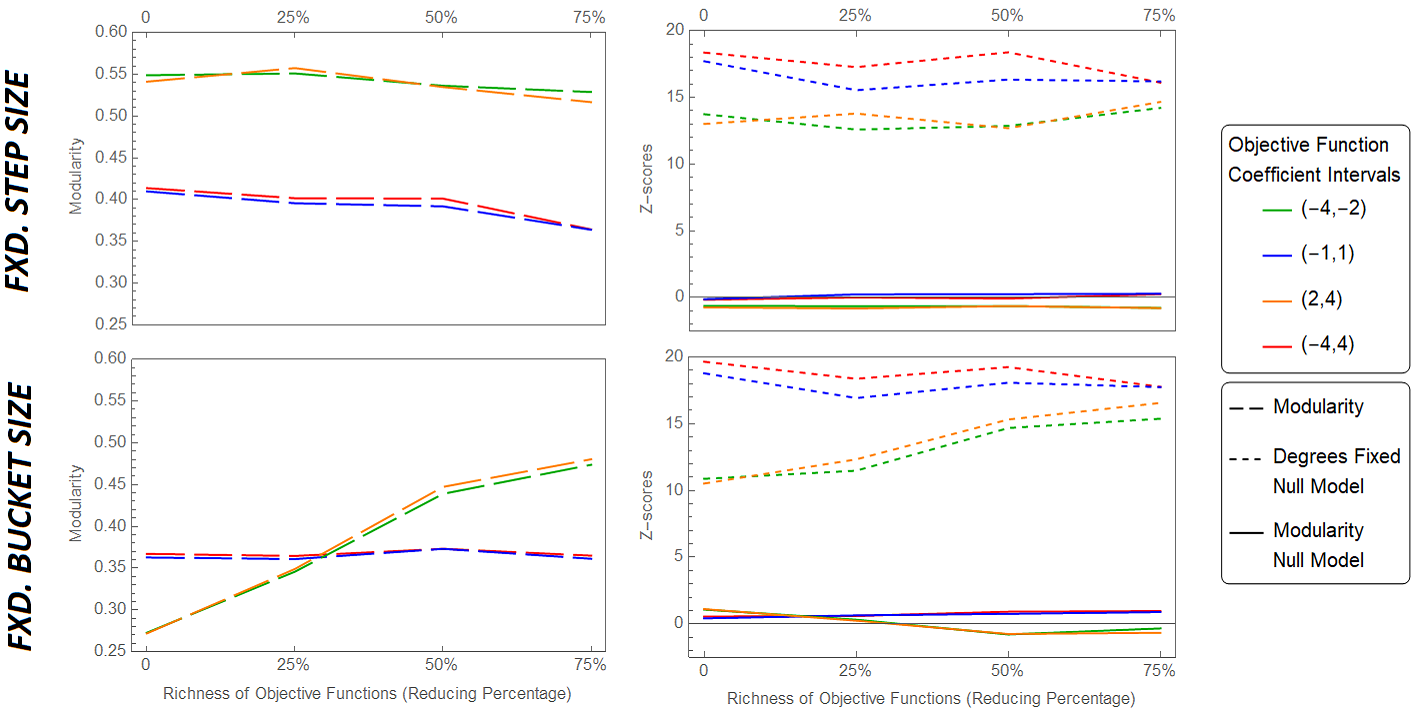
\includegraphics[width=1.03\linewidth]{../images/results-simulation-results.png}}
		\caption{Simulation Analysis Curve Plot Results: Modularity Values and Z-scores.}
		\label{figure-FBA-results}
	\end{center}
\end{figure}

%\begin{equation} %\tag{8}
%	(O.V)_{1}= (o_{1,1}v_{1} + o_{1,2}v_{2} + \dots + o_{1,r}v_{r})
%\end{equation}

%\begin{equation} %\tag{8}
%	(O.V)_{2}= (o_{2,1}v_{1} + o_{2,2}v_{2} + \dots + o_{2,r}v_{r})
%\end{equation}

%\begin{equation} 	
%	(O.V)_{50}= (o_{50,1}v_{1} + o_{50,2}v_{2} + \dots + o_{50,r}v_{r})
%\end{equation}

%\begin{equation} 	
%	(O.V)_{51}= (o_{1,1}v_{1} + o_{1,2}v_{2} + \dots + o_{1,r}v_{r})
%\end{equation}

%\begin{equation} 	
%	(O.V)_{100}= (o_{50,1}v_{1} + o_{50,2}v_{2} + \dots + o_{50,r}v_{r})
%\end{equation}

%\begin{equation} 	
%	(O.V)_{10000}= (o_{50,1}v_{1} + o_{50,2}v_{2} + \dots + o_{50,r}v_{r})
%\end{equation}

%\begin{table}[hb!]
%	\centering
%	\begin{tabular}{|cccccc|l}
%		\cline{1-6}
%		\makecell{Event\\ID} && \makecell{Bio\\Mass} 	&& \makecell{Seq.\\ID} &  \\ \cline{1-6}
%		1 	      && $m_{1}$  	&& 1 		   	&  \\
%		2 		  && $m_{2}$	&& 1 		   	&  \\
%		3 	      && $m_{3}$	&& 2 		    &  \\
%		\vdots	  && \vdots && \vdots 	    &  \\
%		n 		  && $m_{n}$	&& k 		    &  \\ \cline{1-6}
%	\end{tabular}
%	\caption{Arbitrarily Created Data Set $D$.}
%	\label{Tab:D-dataset}
%\end{table}